\documentclass{article}

\usepackage{graphicx}
\usepackage{booktabs}
\usepackage{longtable}
\usepackage{tabu}
\usepackage{listings}
\usepackage{hyperref}

\title{Reporte}

\author{%
stevenpach10
}

\begin{document}

\maketitle

A continuación se presentan los resultados de la métrica accuracy por clase de acuerdo a los datos de prueba del modelo. 

En color verde se representa el modelo que aplica la técnica de upsampling usando 16 de batch. En color gris se representa el modelo que aplica la técnica de upsampling con 32 de batch. En color azul se representa el modelo que sin aplicar upsambling usando 16 de batch. En color morado se representa el modelo que sin aplicar upsambling usando 32 de batch.
\section{Matriz de confusin}

A continuacin se presenta los resultado de la matriz de confusin multiclase normalizados para los cuadro modelos de forma resumida.

\section{Funcin de costo}

A continuacin se presentan la grficas del comportamiento de las funciones de costo para el conjunto de datos de entrenamiento y de pruebas

\begin{figure}[!htb]
\minipage{0.49\textwidth}
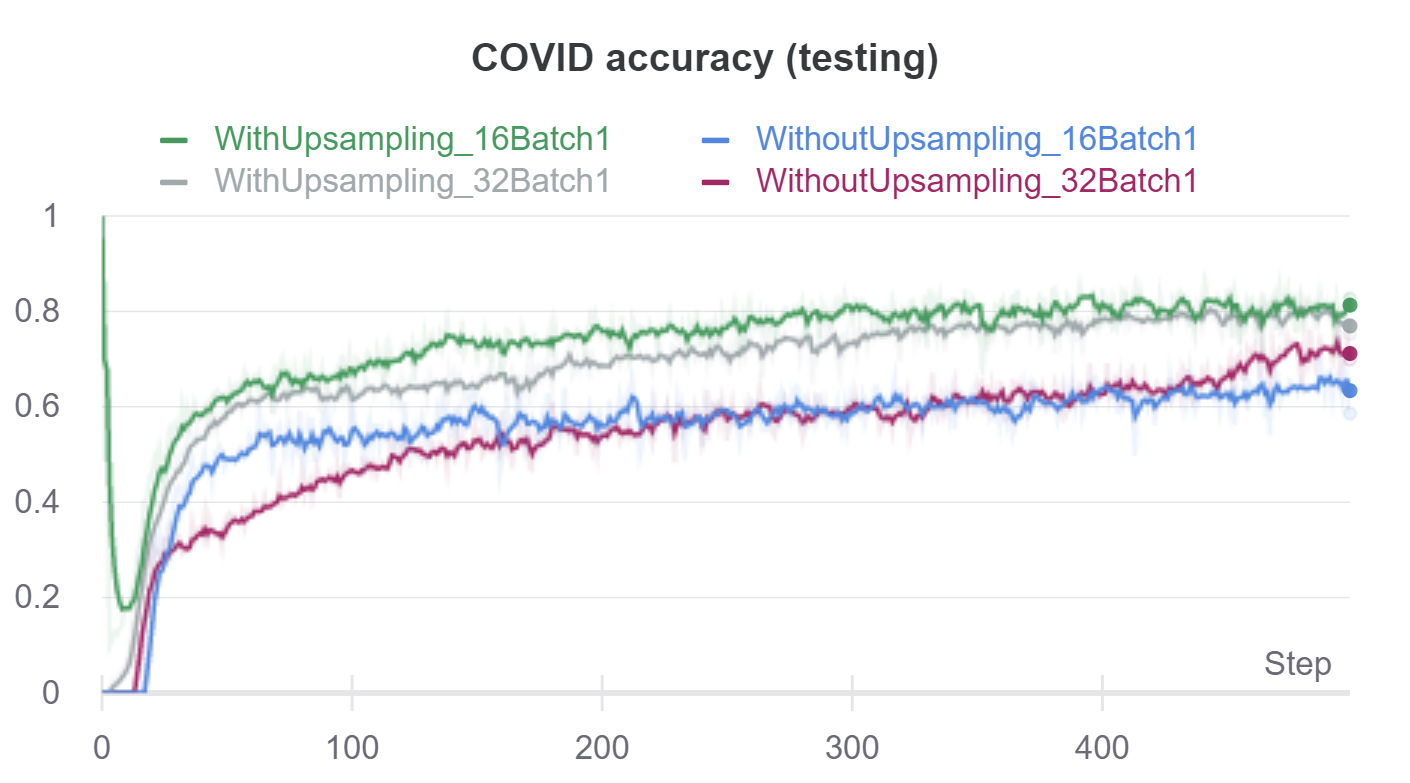
\includegraphics[width=\linewidth]{charts/Section-3-Panel-2-puo6k3y77}
\caption{}
\endminipage\hfill
\minipage{0.49\textwidth}
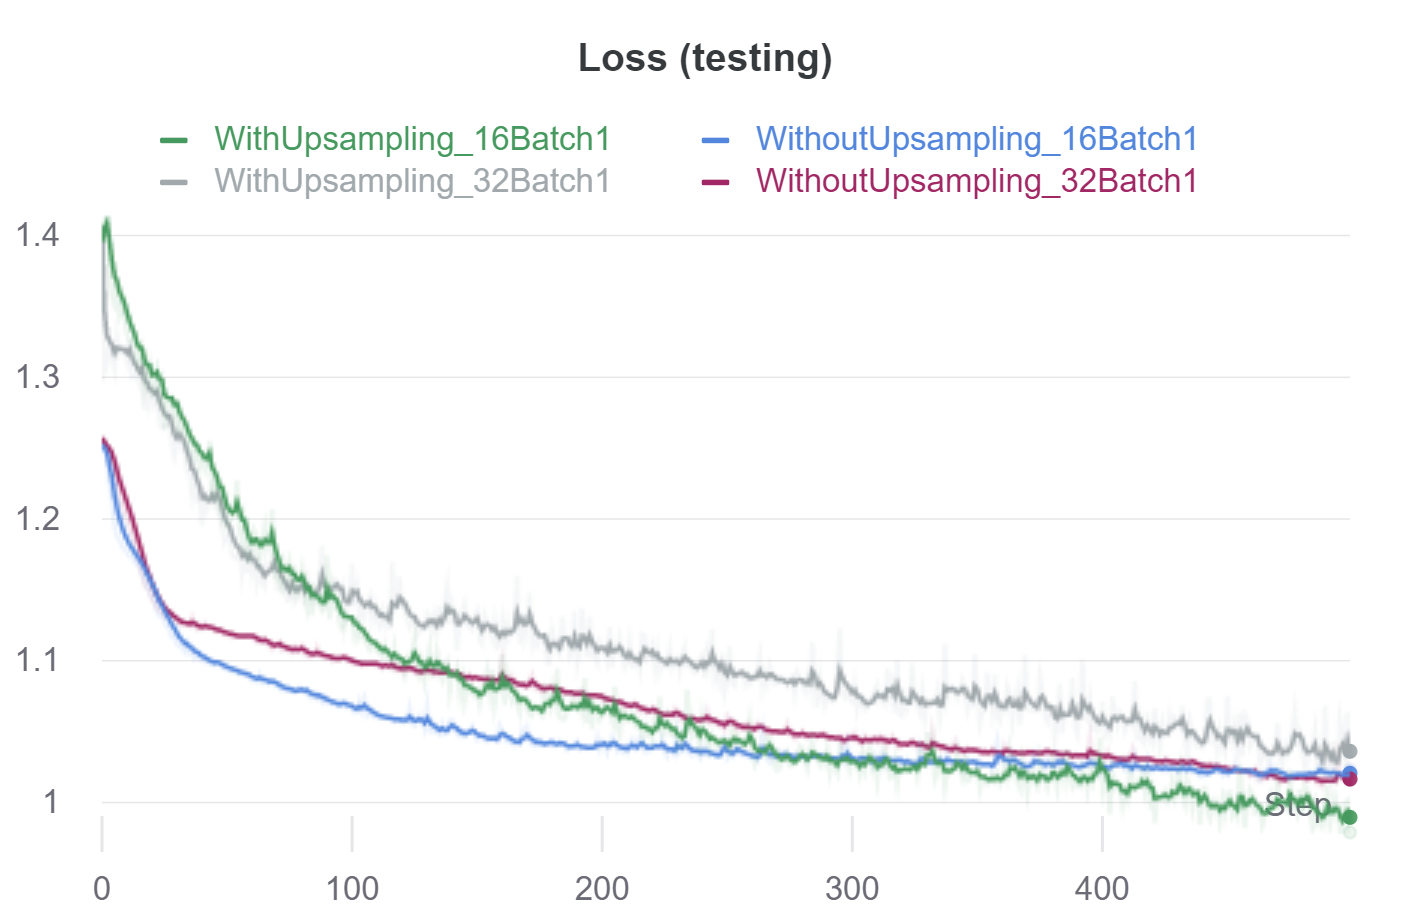
\includegraphics[width=\linewidth]{charts/Section-3-Panel-3-b3qzbvf33}
\caption{}
\endminipage
\end{figure}

\begin{figure}[!htb]
\minipage{0.49\textwidth}
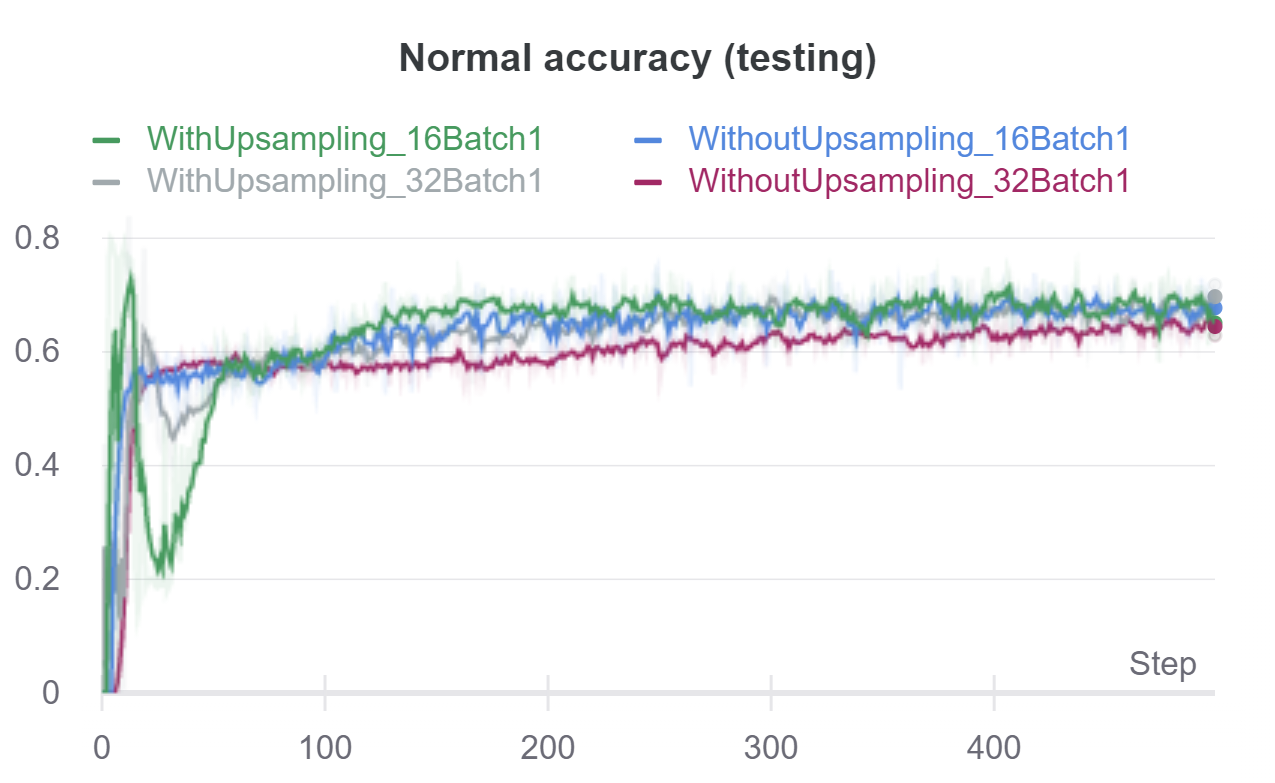
\includegraphics[width=\linewidth]{charts/Section-3-Panel-4-1747d9w1z}
\caption{}
\endminipage\hfill
\minipage{0.49\textwidth}
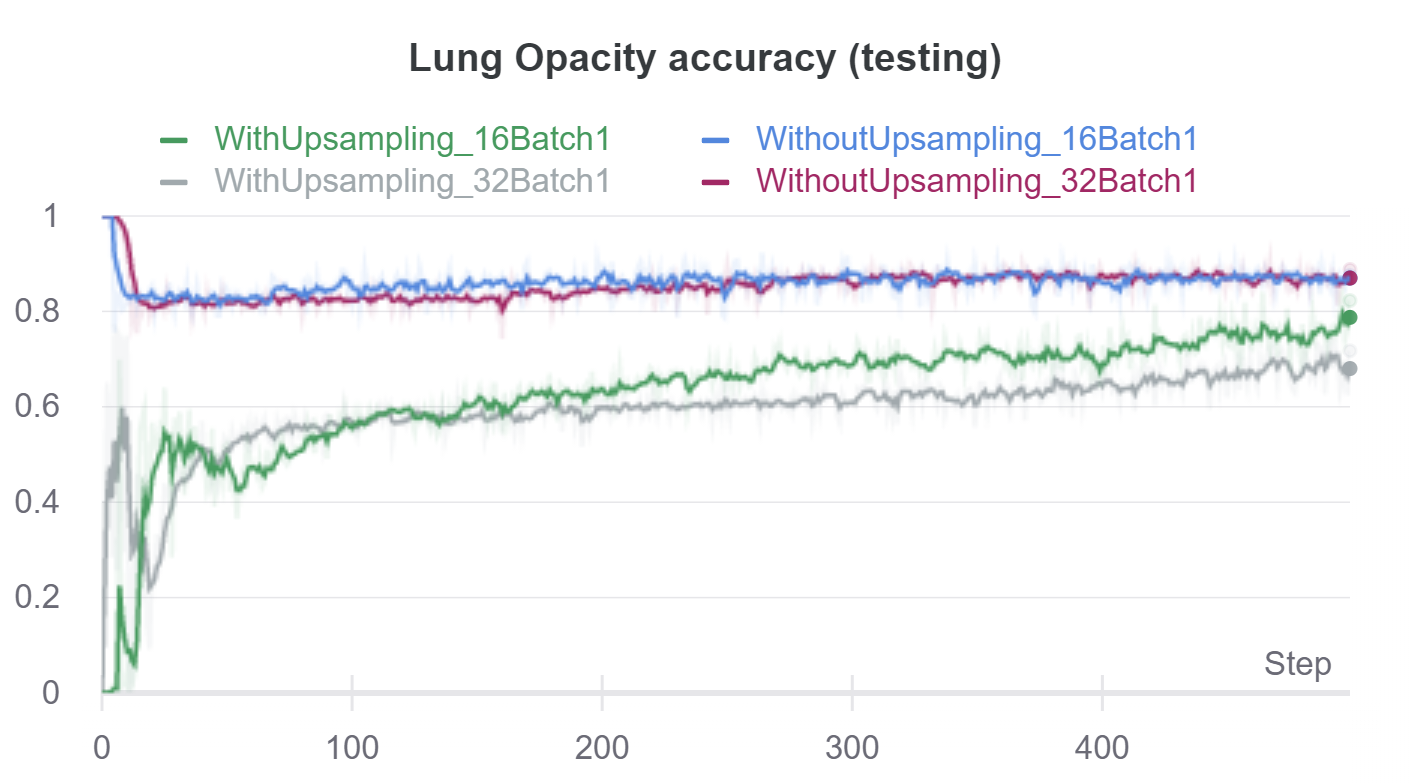
\includegraphics[width=\linewidth]{charts/Section-3-Panel-5-xkatp52si}
\caption{}
\endminipage
\end{figure}

\begin{figure}[!htb]
\minipage{0.49\textwidth}
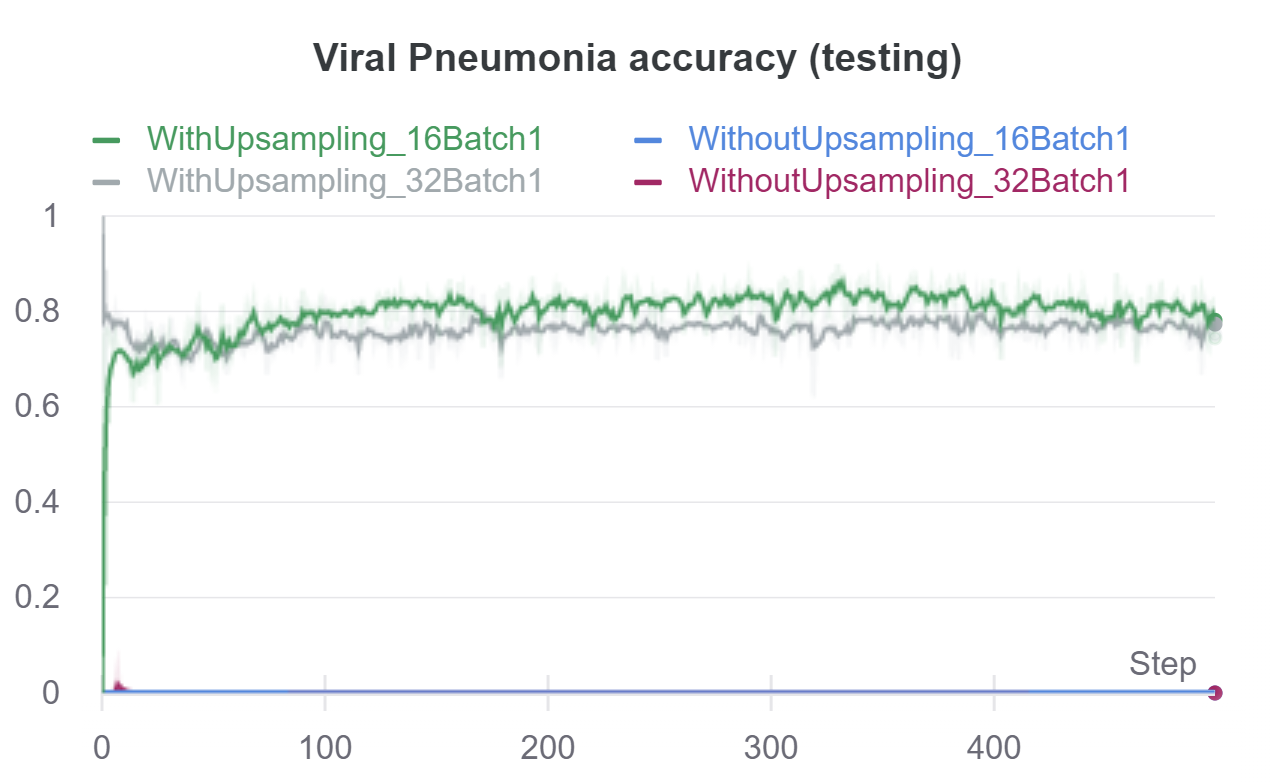
\includegraphics[width=\linewidth]{charts/Section-3-Panel-6-nqd2bkmak}
\caption{}
\endminipage\hfill
\minipage{0.49\textwidth}
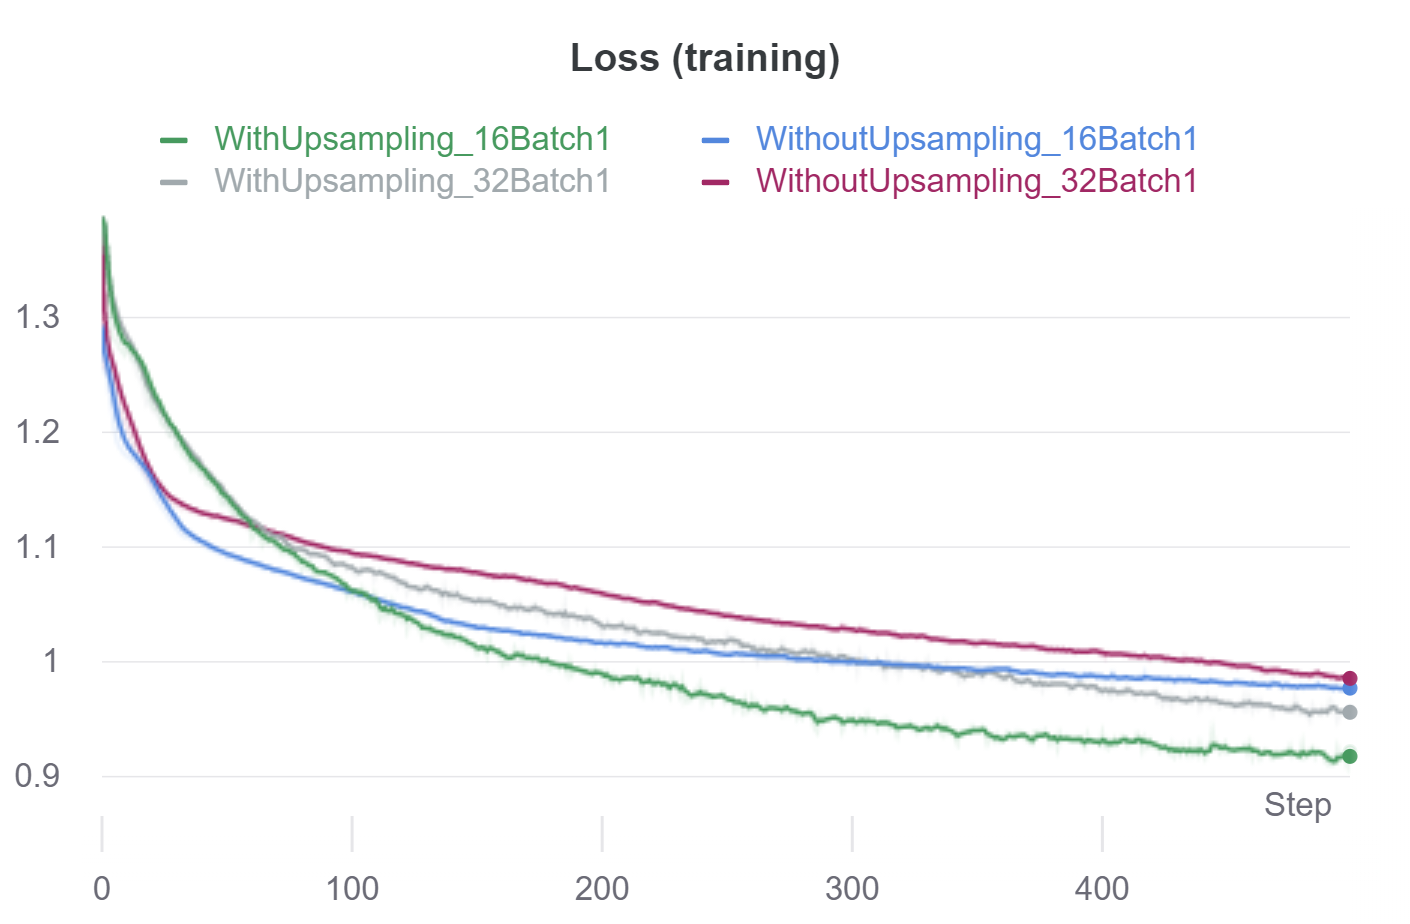
\includegraphics[width=\linewidth]{charts/Section-3-Panel-7-szb5fvuyw}
\caption{}
\endminipage
\end{figure}

\begin{longtabu} spread 0pt {|X[-1]|X[-1]|X[-1]|} \hline
\rowfont[c]{\bfseries}
displayName & state & notes \\ \hline
\rowfont[l]{}
WithUpsampling\_16Batch1 & finished & - \\ \hline
WithoutUpsampling\_16Batch1 & finished & - \\ \hline
WithUpsampling\_32Batch1 & finished & - \\ \hline
WithoutUpsampling\_32Batch1 & finished & - \\ \hline
\end{longtabu}

\nocite{*}
\bibliographystyle{unsrt}
\bibliography{bibliography}
\end{document}